\documentclass[border=10pt]{standalone}
\usepackage[svgnames]{xcolor}
\usepackage{amsmath}
\usepackage{pgfplots}
\pgfplotsset{compat=newest}
\usepackage[sfdefault]{FiraSans}
\usepackage{FiraMono}
\renewcommand*\familydefault{\sfdefault}
\begin{document}
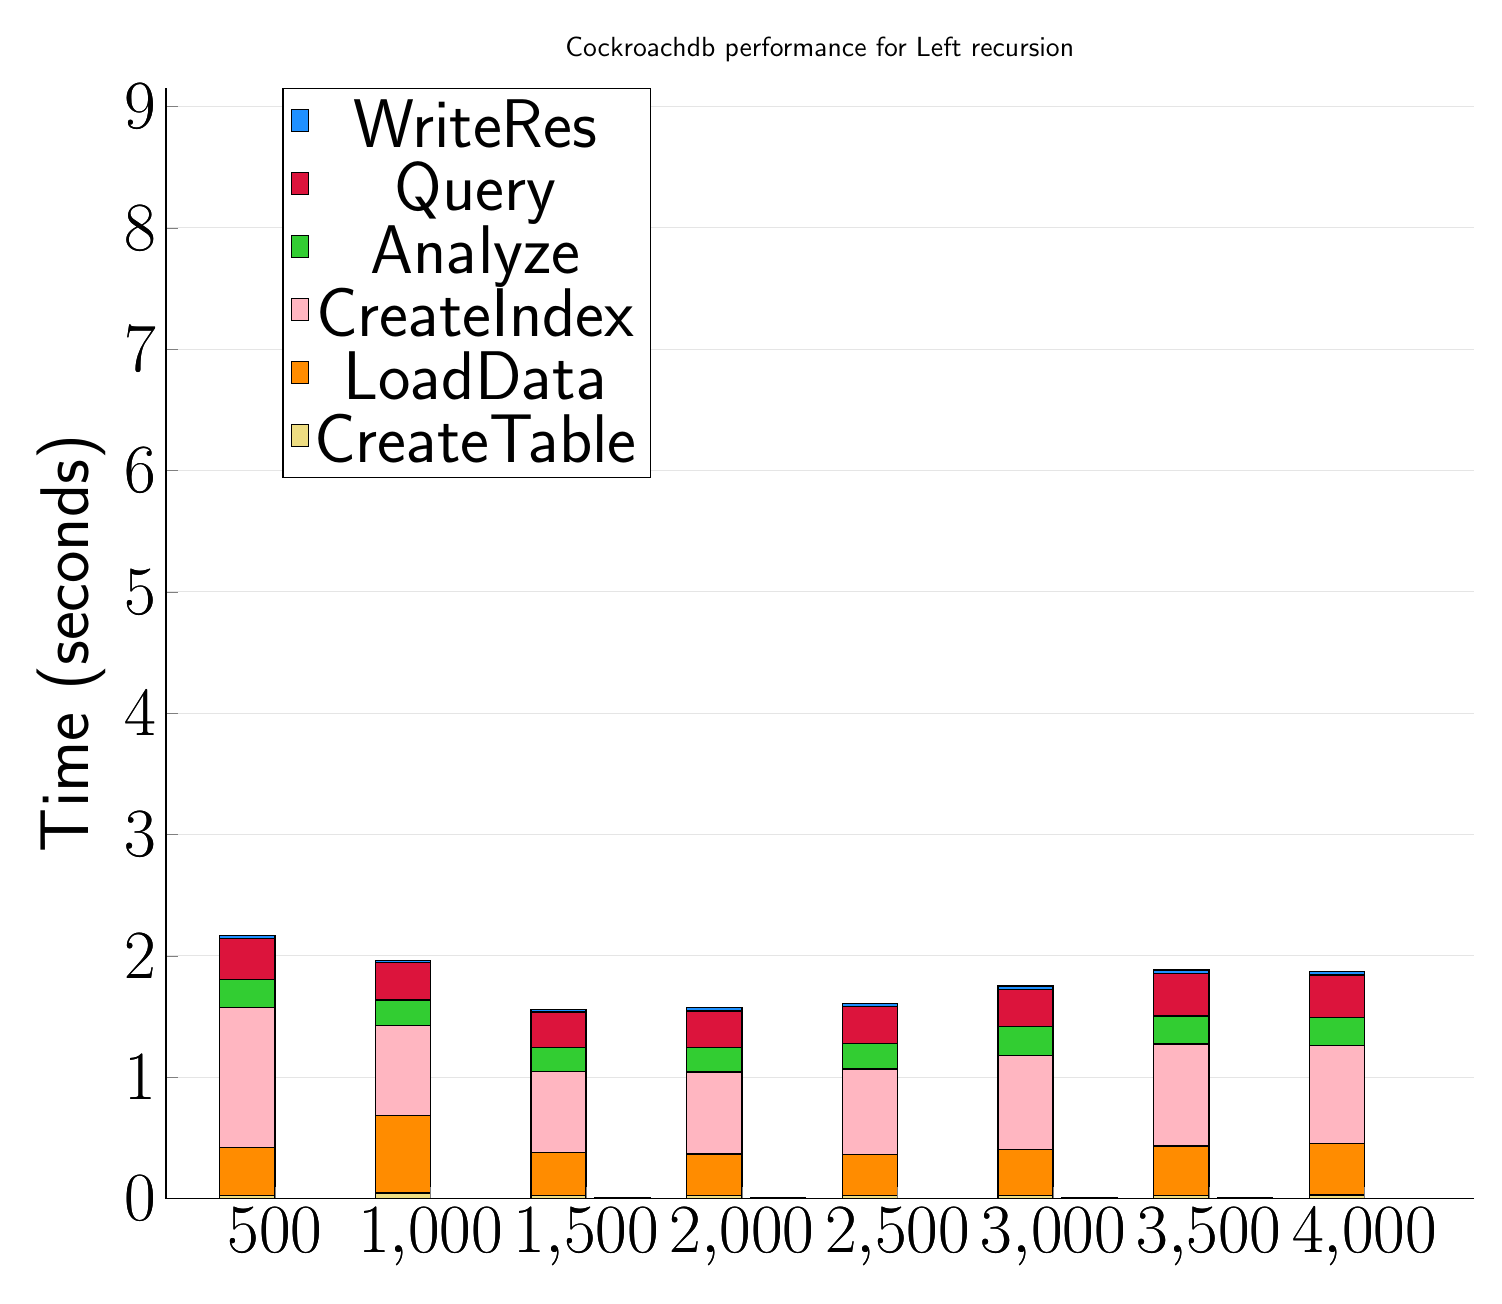
\begin{tikzpicture}
\begin{axis}[
   ybar stacked,
   title={Cockroachdb performance for Left recursion},
   bar shift=-10pt,
   width=1.5\textwidth,
   bar width=0.7cm,
   ymajorgrids, tick align=inside,
   major grid style={draw=gray!20},
   xtick=data,
   ymin=0, ymax=9.153333336114883,
   axis x line*=bottom,
   axis y line*=left,
   enlarge x limits=0.1,
   legend style={
       at={(0.23, 1)},
       anchor=north,
       legend columns=1,
       font=\Huge,
   },
   ylabel={Time (seconds)},
   label style={font=\Huge},
   tick label style={font=\Huge},
]
\addlegendimage{fill=DodgerBlue, draw=black, line width=0.2pt}
\addlegendentry{WriteRes}
\addlegendimage{fill=Crimson, draw=black, line width=0.2pt}
\addlegendentry{Query}
\addlegendimage{fill=LimeGreen, draw=black, line width=0.2pt}
\addlegendentry{Analyze}
\addlegendimage{fill=LightPink, draw=black, line width=0.2pt}
\addlegendentry{CreateIndex}
\addlegendimage{fill=DarkOrange, draw=black, line width=0.2pt}
\addlegendentry{LoadData}
\addlegendimage{fill=LightGoldenrod, draw=black, line width=0.2pt}
\addlegendentry{CreateTable}
\addplot +[fill=LightGoldenrod, draw=black, line width=0.5pt] coordinates {
    (500, 0.026666668554147083)
    (1000, 0.04666666438182195)
    (1500, 0.02333333094914754)
    (2000, 0.023333333432674408)
    (2500, 0.02666666607062022)
    (3000, 0.02666666607062022)
    (3500, 0.026666668554147083)
    (4000, 0.02999999870856603)
};
\addplot +[fill=DarkOrange, draw=black, line width=0.5pt] coordinates {
    (500, 0.39666666587193805)
    (1000, 0.6366666679581007)
    (1500, 0.3566666667660077)
    (2000, 0.34333333373069763)
    (2500, 0.33666666845480603)
    (3000, 0.3799999977151553)
    (3500, 0.40666666626930237)
    (4000, 0.4233333319425583)
};
\addplot +[fill=LightPink, draw=black, line width=0.5pt] coordinates {
    (500, 1.1533333361148834)
    (1000, 0.7433333322405815)
    (1500, 0.6666666641831398)
    (2000, 0.676666667064031)
    (2500, 0.7033333331346512)
    (3000, 0.7733333334326744)
    (3500, 0.8399999986092249)
    (4000, 0.809999999900659)
};
\addplot +[fill=LimeGreen, draw=black, line width=0.5pt] coordinates {
    (500, 0.22999999672174454)
    (1000, 0.20999999841054282)
    (1500, 0.20000000298023224)
    (2000, 0.20333333313465118)
    (2500, 0.21333333353201547)
    (3000, 0.23666666944821677)
    (3500, 0.23000000168879828)
    (4000, 0.22666666408379874)
};
\addplot +[fill=Crimson, draw=black, line width=0.5pt] coordinates {
    (500, 0.33666666597127914)
    (1000, 0.3100000023841858)
    (1500, 0.28999999662240344)
    (2000, 0.29999999950329465)
    (2500, 0.3033333321412404)
    (3000, 0.30666666726271313)
    (3500, 0.34999999900658924)
    (4000, 0.35333333412806195)
};
\addplot +[fill=DodgerBlue, draw=black, line width=0.5pt] coordinates {
    (500, 0.023333333432674408)
    (1000, 0.01666666567325592)
    (1500, 0.023333335916201275)
    (2000, 0.026666668554147083)
    (2500, 0.023333333432674408)
    (3000, 0.02999999870856603)
    (3500, 0.030000001192092896)
    (4000, 0.026666668554147083)
};
\end{axis}
\begin{axis}[
   ybar stacked,
   bar shift=13pt,
   width=1.5\textwidth,
   bar width=0.7cm,
   ymajorgrids, tick align=inside,
   major grid style={draw=none},
   xtick=data,
   ymin=0, ymax=9.153333336114883,
   axis x line*=none,
   axis y line*=none,
   enlarge x limits=0.1,
   label style={font=\Huge},
   tick label style={font=\Huge},
]
\addplot +[fill=LightGoldenrod, draw=black, line width=0.5pt] coordinates {
    (500, 0.0)
    (1000, 0.0)
    (1500, 0.0)
    (2000, 0.0)
    (2500, 0.0)
    (3000, 0.0)
    (3500, 0.0)
    (4000, 0.0)
};
\addplot +[fill=DarkOrange, draw=black, line width=0.5pt] coordinates {
    (500, 0.0)
    (1000, 0.0)
    (1500, 0.0)
    (2000, 0.0)
    (2500, 0.0)
    (3000, 0.0)
    (3500, 0.0)
    (4000, 0.0)
};
\addplot +[fill=LightPink, draw=black, line width=0.5pt] coordinates {
    (500, 0.0)
    (1000, 0.0)
    (1500, 0.0)
    (2000, 0.0)
    (2500, 0.0)
    (3000, 0.0)
    (3500, 0.006666666666666668)
    (4000, 0.0)
};
\addplot +[fill=LimeGreen, draw=black, line width=0.5pt] coordinates {
    (500, 0.0)
    (1000, 0.0)
    (1500, 0.0066666666666666706)
    (2000, 0.006666666666666668)
    (2500, 0.0)
    (3000, 0.0066666666666666706)
    (3500, 0.0)
    (4000, 0.0)
};
\addplot +[fill=Crimson, draw=black, line width=0.5pt] coordinates {
    (500, 0.0)
    (1000, 0.0)
    (1500, 0.0)
    (2000, 0.0)
    (2500, 0.0)
    (3000, 0.0)
    (3500, 0.0)
    (4000, 0.0)
};
\addplot +[fill=DodgerBlue, draw=black, line width=0.5pt] coordinates {
    (500, 0.0)
    (1000, 0.0)
    (1500, 0.0)
    (2000, 0.0)
    (2500, 0.0)
    (3000, 0.0)
    (3500, 0.0)
    (4000, 0.0)
};
\end{axis}
\end{tikzpicture}

\end{document}
